\documentclass[11pt, oneside]{article} 
\usepackage{geometry}
\geometry{letterpaper} 
\usepackage{graphicx}
	
\usepackage{amssymb}
\usepackage{amsmath}
\usepackage{parskip}
\usepackage{color}
\usepackage{hyperref}

\graphicspath{{/Users/telliott/Github/precalculus/fig/}}
% \begin{center} \includegraphics [scale=0.4] {gauss3.png} \end{center}

\title{Fundamental theorem of calculus}
\date{}

\begin{document}
\maketitle
\Large

\begin{quote}Calculus has a long history. Although Newton and Leibniz are credited with the invention of calculus in the late 1600s, almost all the basic results predate them. One of the most important is what is now called the Fundamental Theorem of Calculus (ftc), which relates derivatives to integrals.\end{quote}

\url{https://mathcs.clarku.edu/~ma120/FTC.pdf}

The usual way to begin the study of calculus is to think about the slope of the tangent to a curve at a point.  If the point is some particular value of $x$, say $x=a$, then this is

\[ \lim_{h \rightarrow 0} \ \frac{f(a + h) - f(a)}{h} \]
For any $x$ in the domain of $y=f(x)$, we say that this slope is the limit

\[ \lim_{h \rightarrow 0} \ \frac{f(x + h) - f(x)}{h} \]
We may call this construct by various names such as the derivative of $y$ with respect to $x$, $dy/dx$, or $f'(x)$.  

The notation $dy/dx$ is due to Liebnitz, and $f'(x)$ is due to Lagrange.  For situations where $x$ is a function of time $t$, Newton would write $\dot{x}$, $\ddot{x}$ and so on.  Newton called his method "fluxions", concentrating on derivatives with respect to time.

\[ y = f(x) \]
\[ \frac{dy}{dx} = f'(x) \]
Evaluation of this limit for $f(x) = x^n$, $f(x) = e^x$, and $f(x) = \sin(x)$ then follows.  

Some rules (product rule, chain rule and so on) will be introduced that allow us to calculate derivatives of more complicated functions.  We also learn to keep note of various functions and their derivatives because it is essential to be able to "go backwards."

The inverse of differentiation is integration.  By definition

\[ y = f(x) = \int dy \]
Now
\[ \frac{dy}{dx} = f'(x) \]
\[ dy = f'(x) \ dx \]
\[ y = f(x) = \int dy = \int f'(x) \ dx \]

There is an idea in integration which is really profound.  We already introduced it in previous chapters by considering a ball or solid sphere in 3D space and the outer surface of the ball (technically, that \emph{is} the sphere, but no matter).  As Archimedes showed 2200 years ago, the volume of the sphere is this function of the cube of the radius.

\[ V = f(r) = \frac{4}{3} \pi r^3 \]
The question was:  how does the volume change when the radius changes by a little bit?  The big idea is to realize that the answer is exactly the same as the limit we gave above, it is the derivative of $V$ with respect to $r$.

\[ \frac{d}{dr} V = \frac{dV}{dr} = \frac{d}{dr} \frac{4}{3} \pi r^3 = 4 \pi r^2  \]

It is no accident that this result is the same as the formula for the surface area of the sphere.  Increasing the radius $r$ by a little bit $dr$, the new volume that is added is approximately the surface area $4\pi r^2$ times $dr$, the volume of the shell at the radius $r$.

\[ dV = 4 \pi r^2 \ dr \]

This is a completely general idea.  The way it is usually introduced is to consider the graph of a function $f(x)$ in the plane.

\begin{center} 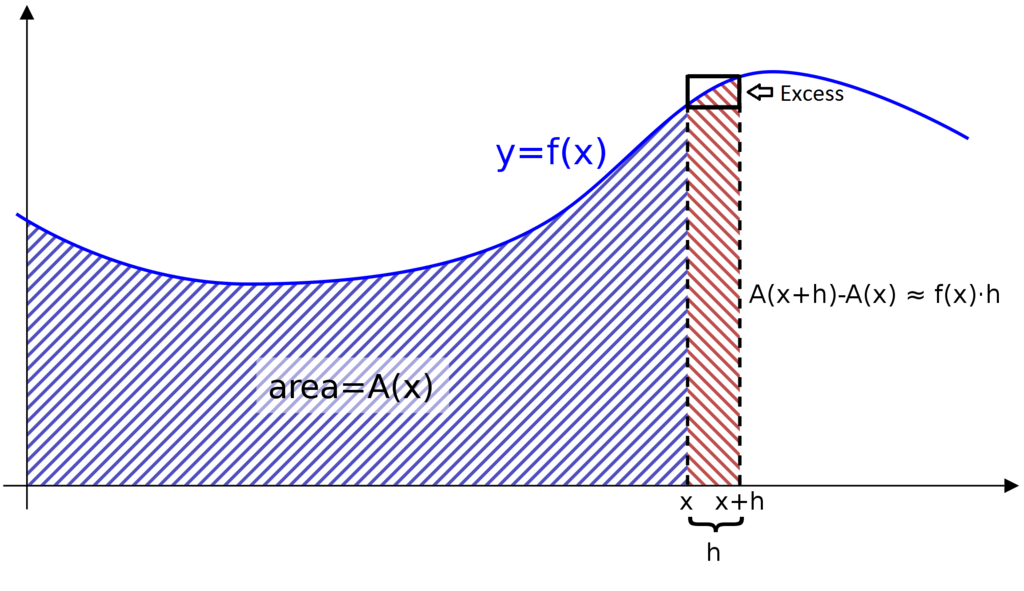
\includegraphics [scale=0.4] {FTC_geometric2.png} \end{center}

We think not just about $f(x)$ itself, but the total area underneath the curve.   Area is a function.  Its value depends on the bounds.  Let us fix the left-hand boundary (say, at $x=a$), but leave the right-hand bound as a variable, call it $x$.  

The big idea is that the total area under the curve (the region in blue) is some as yet unknown function of $x$, $A=F(x)$.  

The way we find $F(x)$ is to ask the question:  how does the area $F(x)$ change when $x$ changes by a little bit, say $h$?  If you look at the figure it is clear that the answer is the area of the red rectangle, the added area is just $f(x)$ times $h$.  If $h$ is small enough, the answer is exact.

Recast in mathematical terms

\[ \lim_{h \rightarrow 0} \ f(x) \ h =  \lim_{h \rightarrow 0} \ F(x + h) - F(x) \]

We just divide by $h$

\[ \lim_{h \rightarrow 0} \ f(x)  =  \lim_{h \rightarrow 0} \ \frac{F(x + h) - F(x)}{h} \]

 and recognize that the term on the left does not depend any longer on $h$ so
 
 \[ f(x)  =  \lim_{h \rightarrow 0} \ \frac{F(x + h) - F(x)}{h} \]

$f(x)$ is the derivative of $F(x)$:

\[ f(x) = F'(x) \]

To find the area function $F$, we just need to find a function that, when we differentiate it, gives us $f(x)$.

The fundamental theorem of calculus states this principle.  Usually, a new variable is introduced to remove any confusion that might arise with respect to $x$, which in the discussion above, we actually used in two different ways.  Write

\[ F(x) = \int_a^x f(t) \ dt \]

In the equation above, the real variable is $x$.  $t$ is what's called a dummy variable, since it might replaced with any other symbol without changing anything.

We have two different functions $F$ and $f$.  The value for each will vary with the value of $x$ (since we evaluate at the right-hand bound $t=x$).  The value of $F$ depends also on the left-hand bound $a$.  Anyway, having written

\[ F(x) = \int_a^x f(t) \ dt \]

The Fundamental Theorem of Calculus (FTC) states:

\[ F'(x) = f(x) \]

which is what we figured out before.

The FTC has a second part, which is

\[ \int_a^b f(x) \ dx = F(b) - F(a) \]

This gives us the way in which areas (and volumes and so on) are actually calculated.  Start with the function $f(x)$.  We find $F(x)$, and then just evaluate it at the endpoints $a$ and $b$.  The difference is the area under the curve $f(x)$ between the two bounds $a$ and $b$.

The proof of this second part is usually done with what are called Riemann sums.  We look at those a bit later in the book.


\end{document}